% !TEX TS-program = pdflatex
% !TEX encoding = UTF-8 Unicode

% This is a simple template for a LaTeX document using the "article" class.
% See "book", "report", "letter" for other types of document.

\documentclass[11pt]{article} % use larger type; default would be 10pt

\usepackage[utf8]{inputenc} % set input encoding (not needed with XeLaTeX)

%%% Examples of Article customizations
% These packages are optional, depending whether you want the features they provide.
% See the LaTeX Companion or other references for full information.

%%% PAGE DIMENSIONS
\usepackage{geometry} % to change the page dimensions
\geometry{a4paper} % or letterpaper (US) or a5paper or....
% \geometry{margin=2in} % for example, change the margins to 2 inches all round
% \geometry{landscape} % set up the page for landscape
%   read geometry.pdf for detailed page layout information

\usepackage{graphicx} % support the \includegraphics command and options

% \usepackage[parfill]{parskip} % Activate to begin paragraphs with an empty line rather than an indent

%%% PACKAGES
\usepackage{booktabs} % for much better looking tables
\usepackage{array} % for better arrays (eg matrices) in maths
\usepackage{paralist} % very flexible & customisable lists (eg. enumerate/itemize, etc.)
\usepackage{verbatim} % adds environment for commenting out blocks of text & for better verbatim
\usepackage{subfig} % make it possible to include more than one captioned figure/table in a single float
% These packages are all incorporated in the memoir class to one degree or another...

\usepackage{amsmath}
\usepackage{algorithm}
\usepackage{algpseudocode}
\usepackage{tikz-qtree}
\usepackage{enumitem}

%%% HEADERS & FOOTERS
\usepackage{fancyhdr} % This should be set AFTER setting up the page geometry
\pagestyle{fancy} % options: empty , plain , fancy
\renewcommand{\headrulewidth}{0pt} % customise the layout...
\lhead{}\chead{}\rhead{}
\lfoot{}\cfoot{\thepage}\rfoot{}

%%% SECTION TITLE APPEARANCE
\usepackage{sectsty}
\allsectionsfont{\sffamily\mdseries\upshape} % (See the fntguide.pdf for font help)
% (This matches ConTeXt defaults)

%%% ToC (table of contents) APPEARANCE
\usepackage[nottoc,notlof,notlot]{tocbibind} % Put the bibliography in the ToC
\usepackage[titles,subfigure]{tocloft} % Alter the style of the Table of Contents
\renewcommand{\cftsecfont}{\rmfamily\mdseries\upshape}
\renewcommand{\cftsecpagefont}{\rmfamily\mdseries\upshape} % No bold!

%%% END Article customizations

\title{Advanced Databases}
\author{ffgt86}
%\date{} % Activate to display a given date or no date (if empty),
         % otherwise the current date is printed 

\begin{document}
\maketitle

\section*{Part A}

\subsection*{a) \textit{Draw the directed tree structure of} \texttt{students.xml}.}

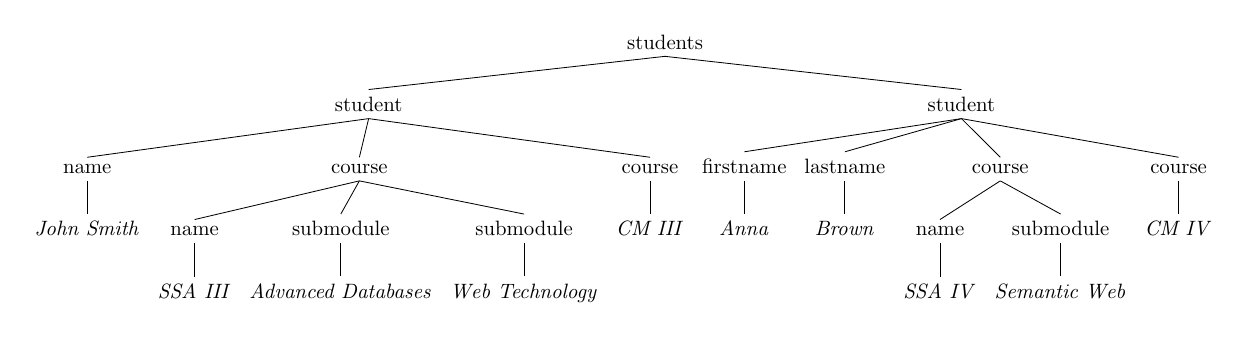
\begin{tikzpicture}[scale=.75]
\Tree[.students
	[.student 
		[.name \textit{John Smith} ]
		[.course 
			[.name \textit{SSA III} ]
			[.submodule \textit{Advanced Databases} ]
			[.submodule \textit{Web Technology} ]
		]
           [.course \textit{CM III} ]
	]
      [.student 
		[.firstname \textit{Anna} ]
		[.lastname \textit{Brown} ]
		[.course
			[.name \textit{SSA IV} ]
			[.submodule \textit{Semantic Web} ]
		]
           [.course \textit{CM IV} ]
	]
]

\end{tikzpicture}

\subsection*{b) \textit{Write a DTD for} teachers.xml.}

This DTD was validated using the \verb|lxml| Python package. The provided file, \verb|teachers.xml|, was modified slightly to facilitate this.

\begin{verbatim}

<?xml encoding="UTF-8"?>
<!ELEMENT teachers (teacher*)>
    <!ELEMENT teacher (name, course*)>
    <!ATTLIST teacher
        jobRole CDATA #REQUIRED
        joiningDate CDATA #REQUIRED>
    <!ELEMENT course (name,submodule+)>
        <!ELEMENT submodule (name,year+)>
            <!ELEMENT year (#PCDATA)>
            <!ELEMENT name (#PCDATA)>

\end{verbatim}

However, with limited examples, and no formal specification, there are ambiguities:

\begin{itemize}

\item{Should a teacher teach at least one course to be included in \verb|teachers.xml|, i.e. \verb|<!ELEMENT teacher (name, course+)>|?}
\item{Should a course contain at least one submodule to be included in \verb|teachers.xml|, i.e. \verb|<!ELEMENT course (name, submodule+)>|?}
\item{Which attributes (if any) are \verb|#REQUIRED|, \verb|#IMPLIED|, or \verb|#FIXED|? Are there default values?}
\item{Are there are limited number of values for \verb|jobRole|? If there were only two roles available, for instance, \verb|Professor| and \verb|Researcher|, the attribute declaration should be \verb|<!ATTLIST teacher jobRole(Professor| $|$ \verb|Researcher)>|.}

\end{itemize}

\subsection*{c) \textit{Is it possible to write a DTD for} \texttt{students.xml}?}

It is not possible. The difficult construct is \verb|<course>|. A student needs one or more courses (\verb|course+|) but a course can either be \verb|#PCDATA| or \verb|(name, submodule*)|, and DTD does not allow mixed delcarations such as \verb|<!ELEMENT course (#PCDATA| $|$ \verb|(name, submodule*)>|. This problem could be eliminated by forbidding \verb|#PCDATA| in \verb|<course>| and always using the \verb|<name>| element, i.e. by changing:

\begin{verbatim}

<student enrolmentDate="2016">
        <firstname>Anna</firstname>
        <lastname>Brown</lastname>
        <course>
            <name>Software, Systems and Applications IV</name>
            <submodule>Semantic Web</submodule>
        </course>
        <course>Computing Methodologies IV</course>
    </student>

\end{verbatim}

to:

\begin{verbatim}

<student enrolmentDate="2016">
        <firstname>Anna</firstname>
        <lastname>Brown</lastname>
        <course>
            <name>Software, Systems and Applications IV</name>
            <submodule>Semantic Web</submodule>
        </course>
        <course>
            <name>Computing Methodologies IV</name>
        </course>
    </student>

\end{verbatim}

The problematic DTD element would then be \verb|<!ELEMENT course (name, submodule*)>|

\clearpage

%%%%%
%PART B%
%%%%%
\section*{Part B}

\verb|XPath| queries were tested using the \verb|lxml| Python package. The provided files, \verb|teachers.xml| and \verb|students.xml|, were modified slightly to facilitate this, and are included in the appendices. \verb|XQuery| queries were tested using an online tool.\footnote{http://videlibri.sourceforge.net/cgi-bin/xidelcgi}

\subsection*{a) \textit{Find all students who study "Advanced Databases" this year.}}

\begin{verbatim}

/students[@year='2019-2020']/descendant::submodule[text()='Advanced Databases']
/ancestor::student

\end{verbatim}

\begin{enumerate}

	\item{Select the \verb|<students>| node with a \verb|year| attribute with value \verb|`2019-2020`| (i.e. this year). There is no need to use the \verb|year| attribute, as there can be only one root element in \verb|students.xml|, but it is included here regardless.}

\begin{center}

	\verb|/students[@year='2019-2020']|

\end{center}

	\item{Select all \verb|<submodule>| descendants from step $1$) with a text value of 'Advanced Databases':}

\begin{center}

	\verb|/descendant::submodule[text()='Advanced Databases']|

\end{center}

	\item{Return the \verb|<student>| ancestors from step $2$):}

\begin{center}

	\verb|/ancestor::student|

\end{center}

\end{enumerate}

The output is:

\begin{verbatim}

<student enrolmentDate="2017">
        <name>John Smith</name>
        <course>
            <name>Software, Systems and Applications III</name>
            <submodule>Advanced Databases</submodule>
            <submodule>Web Technology</submodule>
        </course>
        <course>Computing Methodologies III</course>
    </student>

\end{verbatim}

This approach is robust. Changes to the XML structure, short of removing the \verb|students| or \verb|submodule| elements, are handled by using \verb|descendant| and \verb|ancestor|, rather than hard-coding paths.

\clearpage

\subsection*{b) \textit{Find all teachers who teach "Advanced Databases" this year.}}

\begin{verbatim}

/teachers/descendant::submodule[name='Advanced Databases' and year='2019-2020']
/ancestor::teachers

\end{verbatim}

\begin{enumerate}

	\item{Select all \verb|<submodule>| descendants of \verb|<teachers>| with nodes \verb|<name>| and \verb|<year>| with values 'Advanced Databases' and '2019-2020' (i.e. this year), respectively:} 

\begin{verbatim}

	/teachers/descendant::submodule[name='Advanced Databases' and year='2019-2020']

\end{verbatim}

	\item{Return the \verb|<teacher>| ancestors from step $1$:}

\begin{center}

	\verb|/ancestor::teachers|

\end{center}

\end{enumerate}

The output is:

\begin{verbatim}

<teacher joiningDate="2018" jobRole="Professor">
        <name>Alexandra Cristea</name>
        <course>
            <name>Software, Systems and Applications III</name>
            <submodule>
                <name>Advanced Databases</name>
                <year>2018-2019</year>
                <year>2019-2020</year>
            </submodule>
        </course>
        <course>
            <name>Software, Systems and Applications IV</name>
            <submodule>
                <name>Semantic Web</name>
                <year>2018-2019</year>
                <year>2019-2020</year>
            </submodule>
        </course>
    </teacher>

\end{verbatim}

This approach is similarly robust to part $a$). 

\clearpage
\subsection*{c) \textit{How many years has Professor Cristea been teaching "Advanced Databases" (at Durham)?}}

\begin{verbatim}

xquery version "3.0";

for $t in /teachers/teacher
where $t/name='Alexandra Cristea'

for $s in $t/course/submodule
where $s/name='Advanced Databases'

return count($s/year)

\end{verbatim}

\begin{enumerate}

\item{Select teachers called 'Alexandra Cristea':}

\begin{verbatim}

for $t in /teachers/teacher
where $t/name='Alexandra Cristea'

\end{verbatim}

\item{Select submodules called 'Advanced Databases' taught by \verb|$t| (i.e. Alexandra Cristea):}

\begin{verbatim}

for $s in $t/course/submodule
where $s/name='Advanced Databases'

\end{verbatim}

\item{Return the number of years the submodule \verb|$s| has been taught}:

\begin{verbatim}

return count($s/year)

\end{verbatim}

\end{enumerate}

The output of this query is $2$. If there exists more than one teacher with the name 'Alexandra Cristea', or more than one submodule with the name 'Advanced Databases', this query will sum results. In practice, a teacher or submodule would likely be selected by UID, rather than name, so this should not be an issue. An equivalent \verb|XPath| query can be constructed:

\begin{verbatim}

count(/teachers/teacher[name='Alexandra Cristea']/course
/submodule[name='Advanced Databases']/year)

\end{verbatim}

\clearpage
\subsection*{d) \textit{Find all students in year 3 currently taught by Alexandra.}}

\begin{verbatim}

xquery version "3.0";

for $s in /teachers/teacher[name='Alexandra Cristea']/course/submodule/name

for $k in /students/student[@enrolmentDate='2016']
	where $s=$k/course/submodule

return $k

\end{verbatim}

\begin{enumerate}

\item{Select the names of all submodules \verb|$s| taught by 'Alexandra Cristea':}

\begin{verbatim}

for $s in /teachers/teacher[name='Alexandra Cristea']/course/submodule/name

\end{verbatim}

\item{Return all students \verb|$k| who enrolled in $2016$ (and are thus in their third year) and join \verb|$s| with \verb|$k| on \verb|$k/course/submodule|. This join only selects students who study submodules that 'Alexandra Cristea' teaches.}

\begin{verbatim}

for $k in /students/student[@enrolmentDate='2016']
	where $s=$k/course/submodule

return $k
\end{verbatim}

\end{enumerate}

The outcome of this query is:

\begin{verbatim}

<student enrolmentDate="2016">
        <firstname>Anna</firstname>
        <lastname>Brown</lastname>
        <course>
            <name>Software, Systems and Applications IV</name>
            <submodule>Semantic Web</submodule>
        </course>
        <course>Computing Methodologies IV</course>
    </student>

\end{verbatim}

The same issues as listed in part \textit{c}) affect this query. Additionally, it is not clear whether the \verb|<course>| elements in \verb|<student>| contain courses studied \textit{this year} or in previous years. If the latter is the case, the query becomes significantly more complex. No equivalent \verb|XPath| query can be constructed, as there is no mechanism to 'join' documents, as is used here in step $2$.

\subsection*{e) \textit{How many teachers and how many students are kept in the databases where the last name is not known?}}

This question is ambiguous:

\begin{enumerate}

\item{Does it refer to teachers and students with no \verb|<lastname>| element, those with only a single name in a \verb|<name>| element, or both?}. The former is assumed.
\item{Does it require \textit{two} results, one the number of teachers missing last names, and one the number of students missing last names, or their sum? The latter is assumed.}

\end{enumerate}

\begin{verbatim}

xquery version "3.0";

for $t in /teachers/teacher
	where not(exists($t/lastname))
    
for $s in /students/student
    where not(exists($s/lastname))

return count($t) + count($s)

\end{verbatim}

\begin{enumerate}

\item{Select teachers \verb|$t| without a \verb|<lastname>| element:}

\begin{verbatim}

for $t in /teachers/teacher
	where not(exists($t/lastname))

\end{verbatim}

\item{Select students \verb|$s| without a \verb|<lastname>| element:}

\begin{verbatim}

for $t in /teachers/teacher
	where not(exists($t/lastname))

\end{verbatim}

\item{Return the sum of the number of elements in \verb|$t| and \verb|$s|}:

\begin{verbatim}

return count($t) + count($s)

\end{verbatim}

\end{enumerate}

No \textit{single} equivalent XPath query can be constructed, as it is not possible to query two different documents in one query, but the results from two could easily be summed.

\clearpage
\section*{Appendices}
\subsection*{The modified \texttt{students.xml}}

\begin{verbatim}

<?xml version='1.0' standalone='yes'?>
<students year="2019-2020">
    <student enrolmentDate="2017">
        <name>John Smith</name>
        <course>
            <name>Software, Systems and Applications III</name>
            <submodule>Advanced Databases</submodule>
            <submodule>Web Technology</submodule>
        </course>
        <course>Computing Methodologies III</course>
    </student>
    <student enrolmentDate="2016">
        <firstname>Anna</firstname>
        <lastname>Brown</lastname>
        <course>
            <name>Software, Systems and Applications IV</name>
            <submodule>Semantic Web</submodule>
        </course>
        <course>Computing Methodologies IV</course>
    </student>
</students>

\end{verbatim}

\clearpage
\subsection*{The modified \texttt{teachers.xml}}


\begin{verbatim}

<?xml version="1.0" standalone="no"?>
<teachers>
    <teacher joiningDate="2018" jobRole="Professor">
        <name>Alexandra Cristea</name>
        <course>
            <name>Software, Systems and Applications III</name>
            <submodule>
                <name>Advanced Databases</name>
                <year>2018-2019</year>
                <year>2019-2020</year>
            </submodule>
        </course>
        <course>
            <name>Software, Systems and Applications IV</name>
            <submodule>
                <name>Semantic Web</name>
                <year>2018-2019</year>
                <year>2019-2020</year>
            </submodule>
        </course>
    </teacher>
</teachers>

\end{verbatim}

\end{document}
